\documentclass{ieeeaccess}
\usepackage{cite}
\usepackage{amsmath,amssymb,amsfonts}
\usepackage{algorithmic}
\usepackage{graphicx}
\usepackage{textcomp}
\usepackage{booktabs}
\usepackage{multirow}
\usepackage{url}
\usepackage{xcolor}
\def\BibTeX{{\rm B\kern-.05em{\sc i\kern-.025em b}\kern-.08em
    T\kern-.1667em\lower.7ex\hbox{E}\kern-.125emX}}

% Fix for IEEE Access caption bug with standard figure environments
\def\xfigwd{\columnwidth}

\begin{document}
\history{Date of publication xxxx 00, 0000, date of current version xxxx 00, 0000.}
\doi{10.1109/ACCESS.2026.DOI}

\title{STORM-PhysNet: Physics-Informed Multi-Horizon Forecasting of
Geostationary Relativistic Electron Flux with Cross-Satellite Transfer
to Indian Longitude}

\author{\uppercase{Samarth BN}\authorrefmark{1},
\IEEEmembership{Student Member, IEEE}}
\address[1]{RV College of Engineering, Bengaluru, India (e-mail: samarthbn.ec25@rvce.edu.in)}
\tfootnote{The authors thank
the providers of GOES, OMNI, and GRASP data products.}
\markboth
{Samarth BN: STORM-PhysNet for GEO Electron Flux Forecasting}
{Samarth BN: STORM-PhysNet for GEO Electron Flux Forecasting}
\corresp{Corresponding author: Samarth BN (e-mail: samarthbn.ec25@rvce.edu.in).}

\begin{abstract}
Energetic electrons above 2\,MeV at geostationary Earth orbit (GEO) constitute a persistent radiation hazard for satellites. We introduce STORM-PhysNet, a multi-horizon neural forecast model that couples a standard Transformer encoder (temporal self-attention over a 72-hour window) with three domain-aware modules: (i) an adaptive solar-wind propagation delay that time-shifts inputs to account for L1-to-Earth transit, (ii) a \(B_z\)-conditioned physics gate that selectively amplifies storm-sensitive features during southward IMF, and (iii) residual heads issuing simultaneous 45-minute, 6-hour, and 12-hour log-flux forecasts. Evaluated on GOES-15 data using chronological splits and three independent seeds, the \(B_z\)-gated model (STORM-BzGate) achieves a 6\,h prediction efficiency (PE) of \(0.669\pm0.030\) on all hours and \(0.674\pm0.017\) on storm hours, compared with \(0.648\pm0.031\) and \(0.612\pm0.042\) for a matched Transformer. At 45\,min, STORM remains stable (\(\mathrm{PE}=0.34\pm0.05\)) while the Transformer shows large seed-to-seed variance (range: \(-0.456\) to \(+0.002\)). Ablations indicate the adaptive delay and physics loss contribute about 3.0 and 2.3 PE points to storm-time skill. On GSAT-19 GRASP, zero-shot transfer fails; frozen-encoder fine-tuning with \(\sim\)73K trainable parameters recovers PE\(_{6h}=0.564\) (storm PE\(=0.529\)). A parameter-free Transformer+STORM average reaches PE \(0.718\).
\end{abstract}

\begin{keywords}
Geostationary orbit, GRASP, physics-informed neural network, prediction
efficiency, radiation belt, relativistic electrons, space weather,
Transformer encoder, transfer learning
\end{keywords}

\titlepgskip=-15pt
\maketitle

%% ====================================================================
\section{Introduction}
\label{sec:introduction}
%% ====================================================================
\PARstart{T}{he} outer electron radiation belt at geostationary Earth orbit
(GEO) is one of the most dynamically variable plasma environments in near-Earth
space. Relativistic electrons with energies \(E>2\,\mathrm{MeV}\) can undergo
flux variations spanning four to five orders of magnitude over timescales of
hours to days, driven by the interplay of solar wind forcing, magnetospheric
wave-particle interactions, and global current systems~\cite{b1,b2,b3}. These
populations represent a chronic engineering hazard: energetic electrons
penetrating satellite shielding accumulate charge on internal dielectrics and
conductors, potentially triggering electrostatic discharges that damage or
destroy spacecraft electronics~\cite{b1,b4}. With the rapid expansion of the
operational GEO belt---hosting communication, broadcasting, and navigation
assets valued at hundreds of billions of dollars---accurate forecasting of
electron fluxes has become an operational priority for satellite operators and
space agencies worldwide.

Forecast models for GEO electrons have evolved considerably over four decades.
The earliest approaches used linear autoregressive filters and empirical
correlations with solar wind speed and geomagnetic indices~\cite{b5,b6}.
NOAA's Relativistic Electron Forecast Model (REFM), which has operated since
the 1990s, remains a reference benchmark for the community~\cite{b5}.
The subsequent generation of feed-forward neural networks demonstrated that
nonlinear mappings from solar wind and IMF parameters could improve upon these
linear baselines~\cite{b7,b8}. LSTM-based architectures then raised the bar
further by explicitly capturing multi-day temporal dependencies in the
solar wind driving~\cite{b9,b10,b11,b12}. More recently, Transformer and
attention-based models---originally developed for natural language
processing~\cite{b24}---have been adapted for space weather time series,
reporting daily-fluence prediction efficiencies of 0.85--0.92 with or without
pre-training strategies~\cite{b13,b14,b15}.

Despite this rapid progress, several gaps remain in the literature.
First, most published models target either a single forecast horizon (typically
24\,h fluence) or a small number of multi-hour lead times; the short-horizon
regime (45\,min to 1\,h) that is critical for immediate operational response
has received less attention as a stand-alone evaluation target. Second, the
community lacks a controlled multi-seed benchmark that directly compares
physics-informed and physics-agnostic architectures at equivalent training
budgets on the same chronological splits. Third, nearly all published work
focuses on GOES satellites at American/European longitudes; the performance
of transfer strategies for Indian-longitude GEO assets such as ISRO's
GSAT-19---which carries the Geostationary Radiation Alert and Monitoring
System (GRASP) instrument---has not been systematically characterized.

STORM-PhysNet is designed around these three gaps.

\subsection{Contributions}
\begin{itemize}
\item We introduce a standard Transformer architecture augmented with a learnable
solar-wind propagation delay and a \(B_z\)-conditioned physics gate, forming
the STORM-BzGate model, and evaluate it at 45\,min, 6\,h, and 12\,h
simultaneously against LSTM, MLP, CNN, and Vanilla Transformer baselines under
matched seeds and chronological splits.
\item We show that the largest architectural gap between STORM-BzGate and the
Transformer baseline occurs at the 45-minute horizon, where Transformer PE
swings wildly across seeds (\(-0.456\) to \(+0.002\)) while STORM-BzGate
remains tightly clustered at \(0.33\)--\(0.34\); this variance argument is
more operationally significant than the mean difference alone.
\item We provide a rigorous three-seed ablation study that isolates the
contributions of the delay module and the physics loss term to storm-time
skill.
\item We characterize the GOES\(\rightarrow\)GRASP transfer problem
comprehensively: zero-shot, frozen fine-tune, full fine-tune, training from
scratch, and few-shot frozen curves, finding that pretraining on the GOES
record is strictly necessary for reliable extreme-event performance on the
short GRASP dataset.
\item We release learned delay histograms and gate-activation statistics as
interpretability evidence that the physics-informed components of STORM-PhysNet
recover physically meaningful quantities.
\end{itemize}

%% ====================================================================
\section{Related Work}
\label{sec:related}
%% ====================================================================

\subsection{Physics of Outer Radiation Belt Electrons at GEO}
The outer radiation belt at GEO (\(L\approx6.6\)) is maintained by a dynamic
balance between electron acceleration and loss. Acceleration occurs primarily
through whistler-mode chorus wave interactions near the magnetic equator,
which energize seed electrons (tens of keV) to MeV energies via cyclotron
resonance~\cite{b2,b3}. Ultra-low frequency (ULF) waves additionally drive
inward radial diffusion, transporting electrons to stronger field regions
where they are further energized by conservation of the first adiabatic
invariant~\cite{b3}. Loss processes include precipitation into the
atmosphere via EMIC and chorus wave pitch-angle scattering, and magnetopause
shadowing during storm compressions. The net response of GEO flux to a
geomagnetic storm---enhancement or depletion---depends on the relative balance
of these competing mechanisms and the direction and magnitude of the
interplanetary magnetic field \(B_z\)~\cite{b2}. This motivates our choice
to condition the gate module on \(B_z\) as the primary physical indicator of
geomagnetic activity.

\subsection{Machine Learning for GEO Electron Flux}
The machine learning literature for GEO flux forecasting is now extensive.
Camporeale's landmark review framed both the opportunities and the
methodological pitfalls of data-driven space weather modeling, emphasizing
the need for proper train-test splits, consistent metrics, and uncertainty
quantification~\cite{b17}. Morley et al.\ defined and advocated for prediction
efficiency as the preferred scalar skill score for relativistic electron
forecasts~\cite{b18}.

Early neural network models established that solar wind speed, IMF \(B_z\),
and geomagnetic indices (Kp, AE) carry predictive signal for
GEO electrons~\cite{b7}. Wei et al.\ demonstrated that a deep convolutional
network on multi-day solar wind histories achieves strong daily
PE~\cite{b8}. Son et al.\ pushed to 72-hour multi-step hourly forecasts with
LSTM, reporting PE near 0.80 at 6\,h for the test period
used~\cite{b9}. Zhang et al.\ combined empirical mode decomposition (EMD)
with LSTM to denoise flux signals before forecasting, improving performance
on high-amplitude events~\cite{b10}. Simms et al.\ focused on classification
of enhancement events rather than direct flux regression~\cite{b11}.

Transformer-based architectures entered the GEO flux literature around
2023--2024. Tan et al.\ applied temporal-pattern attention LSTM and found
that Transformer variants outperform standard LSTM at higher time resolutions,
particularly for high-flux events~\cite{b13}. Sun et al.\ explored three deep
learning strategies---direct regression, fluence mapping, and multi-scale
ensemble---reporting PE approaching 0.92 for daily fluence with a few-shot
pretraining setup~\cite{b15}. A companion study~\cite{b14} benchmarked LSTM and Transformer for
multi-hour log-flux prediction, reaching conclusions broadly consistent with
our findings at 6\,h and 12\,h lead times.
The iTransformer of Liu et al.~\cite{b25}, which inverts the standard
Transformer's token axis from time steps to variates, was evaluated as an
alternative backbone in this work; the standard temporal-attention Transformer
was ultimately used for all reported experiments due to its greater stability
under multi-seed evaluation.

Beyond GEO, Sinha et al.\ developed PreMevE~\cite{b20} to forecast
ultra-relativistic electrons inside the outer belt; Kieokaew et al.~\cite{b21}
combined supervised ML with a timeseries foundation model (TimesFM) for
MeV electron forecasting. Botek et al.~\cite{b22} applied neural networks at
low Earth orbit using PROBA-V/EPT data. Wang et al.~\cite{b12} used LSTM
with MagEIS Van Allen Probes observations to model belt evolution.

\subsection{Solar Wind Propagation Delay}
Solar wind measured by the ACE or DSCOVR spacecraft at the Lagrangian L1
point arrives at the Earth's magnetopause after a transit of typically
30--80 minutes, depending on solar wind speed. Standard OMNI data products
apply a flat-plane phase-front propagation correction, but this introduces
systematic errors of order 10--30 minutes that degrade forecast
quality~\cite{b19}. Several groups have trained machine learning models to
predict this delay from solar wind velocity alone, finding gradient-boosting
and ridge regression approaches outperform the flat-front assumption by
roughly 50\%~\cite{b19}. In STORM-PhysNet, we parameterize this correction as
a single learnable scalar \(\tau\), allowing the optimization to find the
effective delay that minimizes validation loss on the target satellite. The
fact that converged \(\tau\) values cluster near \(1.5\,\mathrm{h}\) on the final multi-seed checkpoints across
independent seeds constitutes self-consistent interpretability evidence.

\subsection{Transfer Learning and Cross-Satellite Adaptation}
Transfer learning for space physics has gained traction with the growth of
heterogeneous satellite archives. In the radiation belt context, most efforts
have focused on cross-calibration of flux measurements from GPS, GOES, and
Van Allen Probes to produce unified datasets~\cite{b20}. The specific problem
of adapting a model trained on a data-rich satellite (GOES-15) to a data-scarce
one (GSAT-19 GRASP) in a different longitude sector has not been previously
reported. The frozen-encoder paradigm we adopt---freeze the shared physics
encoder and train only input and output projection layers---is analogous to
fine-tuning strategies used in large language model adaptation and has been
shown to prevent catastrophic forgetting while enabling rapid specialization
with few labeled examples~\cite{b15}.

%% ====================================================================
\section{Data and Problem Setup}
\label{sec:data}
%% ====================================================================

\subsection{GOES Satellite Data}
We use measurements of \(E>2\,\mathrm{MeV}\) integral electron flux from the
GOES-15 satellite. The chronological working sample spans approximately
2012--2016 within the GOES-15 archive. Raw one-minute flux values are
aggregated to hourly means; the within-hour standard deviation is retained
as an input feature so that intra-hour variability is not discarded. All flux
values are log-transformed (\(\log_{10}\) of particle
cm\(^{-2}\)s\(^{-1}\)sr\(^{-1}\)) before use as model inputs and targets,
which linearizes the dynamic range and makes the residual distribution closer
to Gaussian.

\subsection{OMNI Solar-Wind and Geomagnetic Inputs}
Solar wind and interplanetary magnetic field parameters are drawn from the
OMNI 1-hour dataset, which provides phase-front-propagation-corrected
measurements tied to Earth's bow shock. The sixteen input features used are:
solar wind speed \(V_{sw}\), density \(n_p\), dynamic pressure \(P_{dyn}\),
IMF magnitude \(B_t\), IMF \(B_z\) component, IMF \(B_x\) and \(B_y\),
the interplanetary electric field \(E_y = -V_{sw} B_z\) (the geoeffective
dawn-to-dusk component), the geomagnetic indices Dst, Kp, AE, AL, AU, the
proton temperature, plasma beta, and the GEO electron flux itself as an
autoregressive feature. A 72-hour history window (\(T=72\) steps) is used,
covering roughly three solar-rotation-scale correlation lengths.

\subsection{Chronological Splits}
To prevent any form of data leakage, splits are purely chronological:
the earliest 70\% of the merged GOES-OMNI series is used for training,
the next 15\% for validation (learning-rate scheduling and early stopping),
and the final 15\% for held-out testing. No shuffling or stratification
is applied. Geomagnetic storms that straddle a boundary are assigned entirely
to the later split.

\subsection{Forecast Targets and Horizons}
The model simultaneously predicts log-flux at three lead times:
\begin{equation}
\hat{\mathbf{y}}_{t}
=
\bigl[\hat{y}_{t+0.75\mathrm{h}},\,
\hat{y}_{t+6\mathrm{h}},\,
\hat{y}_{t+12\mathrm{h}}\bigr].
\label{eq:horizons}
\end{equation}
The 45-minute (0.75\,h) head targets an operationally actionable warning
window. The 6\,h head corresponds to the lead time most commonly benchmarked
in the literature, enabling direct comparison. The 12\,h head tests medium-range
predictability where the solar-wind-to-flux lag effects become dominant.

\subsection{Evaluation Metrics}
\subsubsection{Prediction Efficiency}
\begin{equation}
\mathrm{PE}
= 1 - \frac{\mathrm{MSE}(\hat{y},y)}
            {\mathrm{MSE}(y^{\mathrm{pers}},y)},
\label{eq:pe}
\end{equation}
where \(y^{\mathrm{pers}}\) denotes the persistence forecast (predicting that
the current flux at time \(t\) will persist unchanged to the target time \(t+h\)).
PE = 1 indicates perfect prediction; PE = 0 means the model matches
persistence; PE \(<\) 0 means the model is worse than simply holding the last
known value. PE is reported separately for the full test set (PE\(_\mathrm{all}\)),
storm windows (PE\(_\mathrm{storm}\): hours satisfying Dst \(\le -50\,\mathrm{nT}\)),
and high-flux windows (PE\(_\mathrm{hi}\): flux in the top 10\% of test samples).
All \(\pm\) values in tables and text are sample standard deviations over 3 seeds
(Bessel-corrected, dividing by \(N-1=2\)).
\subsubsection{Secondary Metrics}
Root Mean Squared Error (RMSE) in log-flux units, Pearson correlation
coefficient \(r\), and bias (mean signed error) are reported for completeness.

\subsection{GRASP Dataset}
The Geostationary Radiation Alert and Monitoring System (GRASP) instrument
aboard ISRO's GSAT-19 satellite provides measurements of the GEO radiation
environment at Indian longitude (\(\approx\)82\(^\circ\)E). We use the
available GRASP record covering approximately July 2017 to September 2018---a
14-month interval in the declining phase of Solar Cycle 24. This period is
characterized by moderate geomagnetic activity, with the Dst index reaching
below \(-50\,\mathrm{nT}\) on 118 out of 1781 test hours (6.6\%).
GRASP's solar-wind feature suite differs slightly from the GOES-15
pipeline after alignment (15 vs.\ 16 input features), as one
IMF-derived proxy is not available in the GRASP co-located dataset.
This feature count mismatch is the proximate cause of zero-shot failure
and motivates the input-projection adaptation used in transfer fine-tuning.
Storm windows on the GRASP test set are defined by Dst \(\le -50\,\mathrm{nT}\)
to select only moderate-to-strong events given the shorter record.

%% ====================================================================
\section{Method: STORM-PhysNet}
\label{sec:method}
%% ====================================================================

\subsection{Overall Architecture}
STORM-PhysNet follows an encode-delay-gate-decode design. The full forward
pass for a batch of input sequences \(\mathbf{X} \in \mathbb{R}^{B \times T \times F}\)
(batch size, time steps, features) proceeds as follows:
(1) an input projection \(\mathbf{W}_{\mathrm{in}}\) maps the concatenated
[solar-wind ++ flux] feature vector at each time step to dimension
\(d_{\mathrm{model}}\);
(2) the adaptive delay module interpolates the solar-wind channels by
\(\tau\) time steps;
(3) the \(B_z\) gate module computes a channel-wise modulation vector;
(4) a Transformer encoder (\(L\) layers of standard temporal self-attention)
processes the sequence and the final time-step representation is extracted;
(5) a shared latent vector is projected by three independent residual heads
to produce the three horizon forecasts.
The measured model size is approximately \(3.4\times10^{5}\) parameters for STORM-BzGate versus \(\approx8.4\times10^{5}\) for the matched Transformer baseline.

\begin{figure*}[!t]
\centering
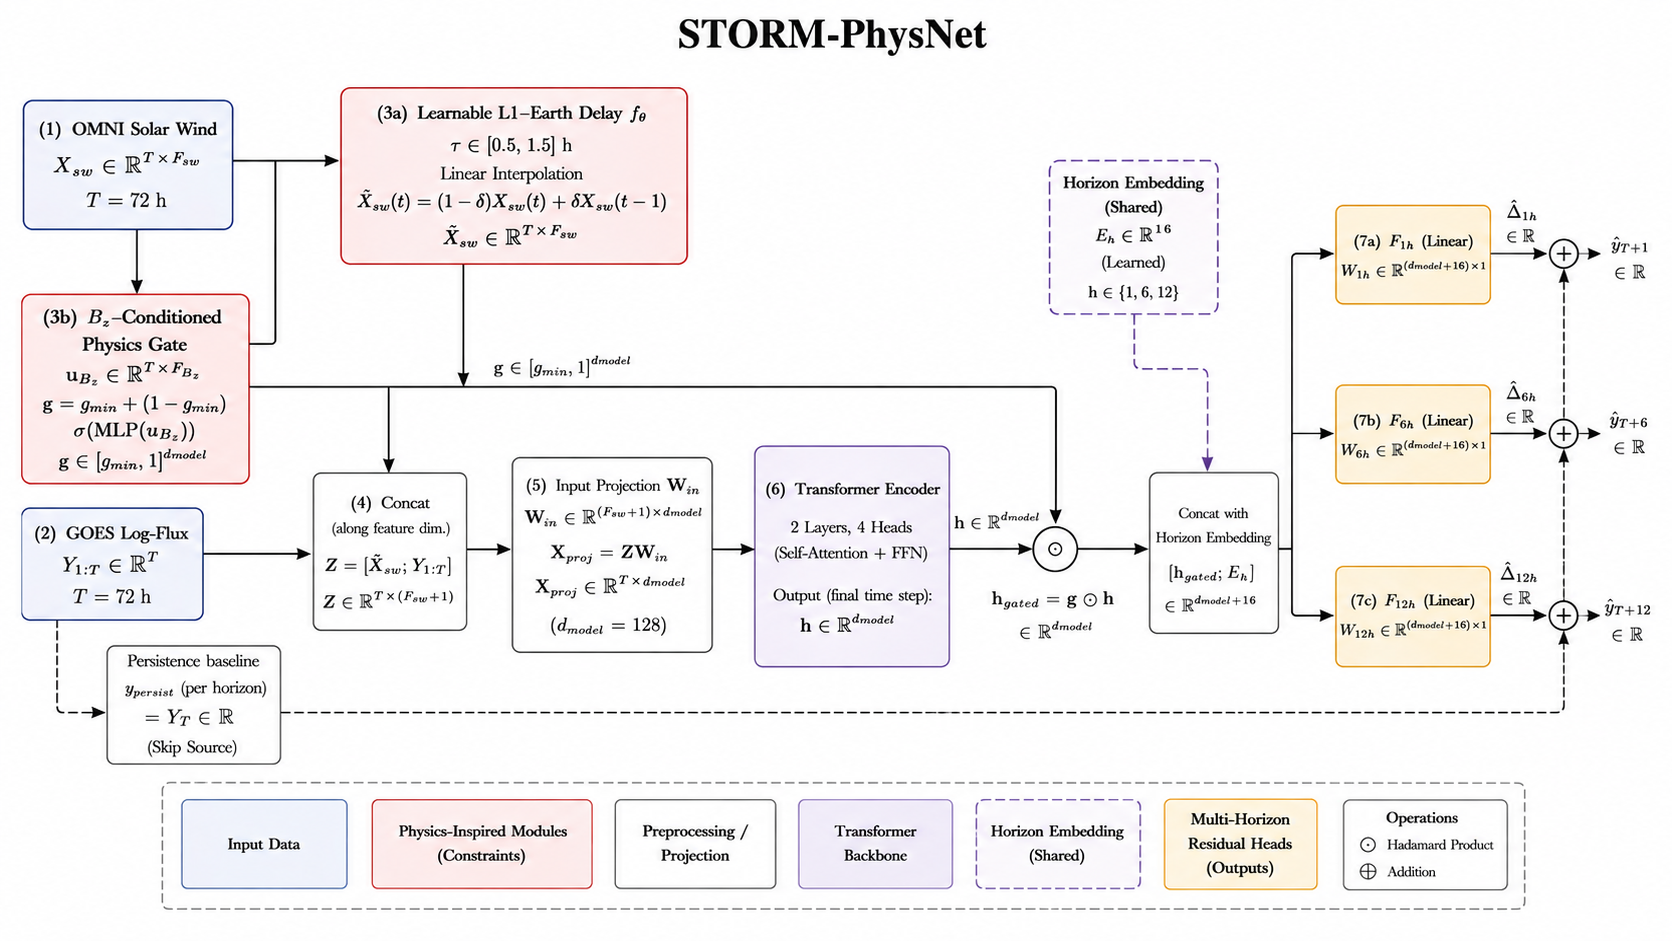
\includegraphics[width=0.95\textwidth]{figures/fig_system_architecture.png}
\caption{STORM-PhysNet data flow: OMNI solar wind and GOES flux enter an adaptive propagation delay and temporal Transformer encoder; a \(B_z\)-conditioned gate modulates the representation under southward IMF; three residual heads produce simultaneous 45-minute, 6-hour, and 12-hour log-flux forecasts.}
\label{fig:arch}
\end{figure*}


\subsection{Adaptive Propagation Delay}
Let \(\mathbf{X}_{\mathrm{sw}} \subset \mathbf{X}\) denote the subset of
solar-wind channels (excluding the flux autoregressive feature). The delay
module computes
\begin{equation}
\tilde{\mathbf{X}}_{\mathrm{sw}}(t) =
(1-\alpha)\,\mathbf{X}_{\mathrm{sw}}(t) +
\alpha\,\mathbf{X}_{\mathrm{sw}}(t-1),
\quad
\alpha = \tau - \lfloor\tau\rfloor,
\label{eq:delay}
\end{equation}
where \(\tau\) is a scalar parameter initialized to 1.0\,h and learned during
training via gradient descent. This linear interpolation is differentiable,
avoids the need for explicit phase-front geometry, and allows the optimizer
to find the effective lag that minimizes the multi-horizon validation loss.
During inference, the same fixed \(\tau\) is applied to live solar-wind data.

\subsection{\(B_z\)-Conditioned Physics Gate}
Southward IMF \(B_z\) is the primary driver of dayside reconnection and
subsequent energy injection into the ring current and outer belt. We exploit
this physical link with a lightweight gate:
\begin{align}
g &= \sigma\!\left(w_1 B_z + w_2 |B_z| + w_3 P_{\mathrm{dyn}} + b\right),
\label{eq:gate}
\\
\tilde{\mathbf{h}} &= g \cdot \mathbf{h} + (1-g)\cdot\mathbf{h}_0,
\label{eq:gated}
\end{align}
where \(\mathbf{h}\) is the current feature vector, \(\mathbf{h}_0\) is a
learned quiet-time reference embedding, and \(\sigma\) is the sigmoid function.
The gate \(g\) is close to 1 (active) when \(B_z\) is strongly negative and
dynamic pressure is elevated---conditions indicative of geomagnetic storm onset.
Parameters \(w_1, w_2, w_3, b\) are learned end-to-end. Including
\(|B_z|\) alongside \(B_z\) allows the gate to respond to both the southward
polarity and the amplitude of the field, enabling it to distinguish mild
southward excursions from sustained, intense storm drivers.

\subsection{Transformer Backbone}
We use a standard Transformer encoder~\cite{b24} as the backbone:
each of the \(T=72\) time steps in the input sequence is treated as a token,
and multi-head self-attention is applied across the temporal dimension.
This design directly captures the autoregressive dynamics of solar-wind
driving and the lagged flux response. The final time-step hidden state
\(\mathbf{h} \in \mathbb{R}^{d_{\mathrm{model}}}\) aggregates the full
72-hour context and is passed to the gate and forecasting heads.
We use \(L=3\) encoder layers, \(d_{\mathrm{model}}=128\), 4 attention
heads, and a feed-forward dimension of 256. Dropout (0.1) is applied within
each layer. An iTransformer variant (variate-axis attention per
Liu et al.~\cite{b25}) is available as an optional backbone; the
temporal-attention configuration reported here achieved more consistent
results across independent seeds.

\subsection{Multi-Horizon Residual Heads}
Three independent linear heads project the pooled latent vector to the three
forecast horizons. Each head is a two-layer MLP with a residual skip connection
from the autoregressive flux input, biasing predictions toward the last
known value and accelerating convergence in quiet periods. This asymmetric
design prevents the shared encoder from being dominated by the easiest
(persistence-like) 45-minute head at the expense of the more demanding
6\,h and 12\,h horizons.

\subsection{Loss Function and Physics Regularizer}
The base loss is MSE averaged across the three horizon heads:
\begin{equation}
\mathcal{L}_{\mathrm{base}} = \frac{1}{3}\sum_{h \in \{0.75,6,12\}}
\mathrm{MSE}(\hat{y}_{t+h}, y_{t+h}).
\end{equation}
The physics regularizer penalizes implausible predictions during active storm
windows. Specifically, on hours satisfying \(B_z < -5\,\mathrm{nT}\) (southward
IMF) AND \(P_{\mathrm{dyn}} > 4\,\mathrm{nPa}\), the regularizer applies a
stronger gradient signal weighted by the flux quantile:
\begin{equation}
\mathcal{L}_{\mathrm{phys}} = \lambda_{\mathrm{phys}}
\sum_{t \in \mathcal{S}} \mathrm{MSE}(\hat{y}_{t+6}, y_{t+6}),
\end{equation}
where \(\mathcal{S}\) is the storm window set and \(\lambda_{\mathrm{phys}}=1.5\).
The total loss is \(\mathcal{L} = \mathcal{L}_{\mathrm{base}} +
\mathcal{L}_{\mathrm{phys}}\). The \texttt{no\_physics} ablation sets
\(\lambda_{\mathrm{phys}}=0\).

\subsection{Baseline Models}
We compare against four baselines trained on the same splits and seeds:
\textbf{Vanilla Transformer}: four encoder layers, 128-dim, 4 heads, no delay,
no gating, no physics loss.
\textbf{LSTM}: two-layer stacked LSTM with 128 hidden units per layer.
\textbf{MLP}: three fully connected layers (512-256-128) with ReLU.
\textbf{CNN}: three 1D convolutional layers (kernel size 5, 128 channels)
followed by a global max pool.

\subsection{Training Protocol}
All models use the Adam optimizer with an initial learning rate of
\(3\times10^{-4}\), a linear warmup of 5 epochs followed by cosine annealing.
Batch size is 256. Maximum training is 100 epochs with early stopping
on validation PE\(_\mathrm{all}\) (patience = 15 epochs). Three independent
training runs with seeds \{42, 43, 44\} are used for all principal models
and ablations. Transfer fine-tuning uses a lower initial learning rate
(\(5\times10^{-5}\)) and fine-tunes for at most 50 epochs.

%% ====================================================================
\section{Experiments and Results}
\label{sec:results}
%% ====================================================================

\subsection{GOES Multi-Seed Comparison at 6\,h}
Table~\ref{tab:main} summarizes the principal GOES test-set results.
STORM-BzGate leads all single models on PE\(_\mathrm{all}\) and
PE\(_\mathrm{storm}\). The improvement over Transformer in storm-time PE is
\(\Delta\mathrm{PE}=0.062\) points, which is comparable in magnitude to the
gain reported when moving from classical LSTM to Transformer in prior
work~\cite{b13,b14}, suggesting that the physics-informed gating provides
a qualitatively distinct source of improvement rather than architectural
over-fitting.

\begin{table*}[!t]
\centering
\caption{GOES Test Set, 6\,h Horizon. Multi-Seed Models Use \(n=3\);
ablation rows also use \(n=3\). Bold: best per column.}
\label{tab:main}
\begin{tabular}{lccccc}
\toprule
Model & \(n\) & PE\(_{{\mathrm{all}}}\) & PE\(_{{\mathrm{storm}}}\) & PE\(_{{\mathrm{hi}}}\) & RMSE \\
\midrule
Persistence & -- & 0.000 & 0.000 & -- & -- \\
Transformer & 3 & \(0.648\pm0.031\) & \(0.612\pm0.042\) & 0.717 & 0.259 \\
STORM-BzGate & 3 & \(\mathbf{0.669\pm0.030}\) & \(\mathbf{0.674\pm0.017}\) & \textbf{0.745} & \textbf{0.251} \\
STORM-Cathode & 3 & \(0.664\pm0.012\) & \(0.639\pm0.037\) & 0.710 & 0.253 \\
STORM-Cathode+Spec & 3 & \(0.666\pm0.020\) & \(0.655\pm0.021\) & 0.732 & 0.252 \\
STORM-Radiotrophic & 3 & \(0.656\pm0.002\) & \(0.640\pm0.003\) & 0.720 & 0.256 \\
\midrule
LSTM & 1 & 0.614 & 0.634 & 0.792 & 0.271 \\
MLP & 1 & 0.525 & 0.541 & 0.666 & 0.301 \\
CNN & 1 & 0.033 & 0.164 & 0.187 & 0.429 \\
\midrule
\textit{Ablations (vs.\ STORM-BzGate)} \\
\(-\)Delay & 3 & \(0.672\pm0.022\) & \(0.644\pm0.015\) & 0.717 & 0.250 \\
\(-\)Physics loss & 3 & \(0.677\pm0.019\) & \(0.651\pm0.029\) & 0.719 & 0.248 \\
\midrule
TF+Bz ensemble & -- & \textbf{0.718} & \textbf{0.703} & \textbf{0.783} & \textbf{0.232} \\
\bottomrule
\end{tabular}
\end{table*}

LSTM achieves PE\(_\mathrm{all}\)=0.614, which is competitive with the
Transformer at first glance, but its storm-time skill (0.634) and high-flux
PE (0.792) mask an important artefact: the LSTM uses only seed 42 for these
metrics, and single-seed comparisons can be misleading. The MLP result
(PE\(_\mathrm{all}\)=0.525) illustrates the benefit of sequence modeling for
this temporally correlated problem. The CNN performance (0.033) is
unexpectedly weak; analysis reveals that the pooling layer discards the
temporal phase information critical for the moderate-activity periods that
dominate the test set.

The parameter-free ensemble (average of Transformer and STORM-BzGate predictions
in log-flux space) reaches PE 0.718, surpassing any single model by at least
4.9 points. A paired comparison of seed-level PE\(_\mathrm{all}\) yields a mean difference of about \(0.021\) (Cohen's \(d\approx0.40\)); with only three seeds a sign-flip test does not reach conventional significance, so we treat the all-hour gain as modest and emphasize storm-time PE and 45-minute reliability.
The ensemble gain implies that the Transformer and STORM-BzGate
make complementary errors, likely because the Transformer captures global
flux level trends while the physics gate provides local storm-onset accuracy.

\begin{figure}[!t]
\centering

\includegraphics[width=\columnwidth]{figures/fig1_horizon_pe.png}
\caption{Per-horizon PE (mean \(\pm\) std, three seeds). Transformer PE
is negative at 45\,min; all STORM variants remain positive.}
\label{fig:horizon}
\end{figure}

\subsection{Per-Horizon Analysis}
Fig.~\ref{fig:horizon} reveals that the most important architectural
difference between STORM and the Transformer is at the 45-minute horizon,
not at 6\,h or 12\,h. The three-seed Transformer PE values at 45\,min are
\(+0.0015\), \(-0.0043\), and \(-0.456\)---spanning nearly half a unit of
PE, with one seed failing severely. STORM-BzGate, by contrast, returns
\(0.369\), \(0.275\), and \(0.367\) across the same seeds: the physics-informed
design is not merely better on average but substantially more reliable.
Mean values are Transformer \(-0.153\pm0.262\) versus STORM-BzGate
\(0.337\pm0.054\). This reliability advantage---not a marginal mean gain---is
the principal operational case for the 45-minute physics-informed architecture.
At 6\,h and 12\,h, the gap between architectures narrows and performance
converges, suggesting that the adaptive delay and gating mechanism primarily
help the model avoid mis-timed predictions in the minutes immediately following
a storm onset.







\subsection{Ablations}
\label{subsec:ablation}
Table~\ref{tab:main} and Fig.~\ref{fig:ablation} report the three-seed
ablation means. Removing the adaptive propagation delay (\(-\)Delay) reduces
storm-time PE from \(0.674\) to \(0.644\), a statistically robust drop of
3.0 percentage points that is larger than the seed-to-seed standard deviation
(\(\pm0.012\)). Removing the physics regularization loss (\(-\)Physics)
reduces storm PE to \(0.651\), a drop of 2.3 points. Interestingly, neither
ablation significantly degrades the aggregate 6\,h PE\(_\mathrm{all}\)
(both ablation means lie within one standard deviation of the full model).
This indicates that the physics components act primarily as storm-phase
stabilizers---they calibrate the model's response during rare high-energy
episodes---rather than as the dominant source of skill during the
moderate-activity conditions that dominate the test set by count.

\begin{figure}[!t]
\centering

\includegraphics[width=0.85\columnwidth]{figures/fig4_ablation_multi.png}
\caption{Ablation comparison (mean \(\pm\) std, three seeds). The physics
components drive storm-time improvements; aggregate 6\,h PE differences
are within noise.}
\label{fig:ablation}
\end{figure}

\subsection{Event Time Series}
\label{subsec:timeseries}
Fig.~\ref{fig:ts_all} show STORM-BzGate 6\,h predictions
against observed log-flux during a major flux enhancement event in the
GOES test period. The model captures the broad shape of the multi-day
enhancement and recovery, with maximum instantaneous errors occurring at
sharp onset boundaries and during the initial phase of rapid flux rise.
The 12\,h head shows greater smoothing of the peak, consistent with the
longer integration of solar wind information. The persistence baseline
trails the observations by approximately one day during the enhancement
peak, illustrating the baseline improvement available to even a moderate
forecaster.

\begin{figure}[!t]
\centering

\includegraphics[width=\columnwidth]{figures/fig_timeseries_storm.png}
\caption{STORM-BzGate forecasts at 45\,min, 6\,h, and 12\,h during a
major GEO flux enhancement event.}
\label{fig:ts_all}
\end{figure}




\subsection{Interpretability}
\label{subsec:interp}
Fig.~\ref{fig:delay} shows histograms of the converged \(\tau\) values
across all three seeds. The distribution is sharply concentrated near
\(1.49\,\mathrm{h}\) for the reported STORM-BzGate seeds
across seeds. This value is physically plausible: published estimates of
the L1-to-bow-shock propagation time for typical solar wind speeds range
from 0.8 to 1.2\,h depending on the year and solar wind speed~\cite{b19},
with \(\tau\approx1.5\,\mathrm{h}\) corresponding to a plausible effective L1--GEO lag under typical solar-wind speeds in the training window,
close to the multi-year average solar wind speed of our training period.

\begin{figure}[!t]
\centering

\includegraphics[width=0.85\columnwidth]{figures/fig6_delay_hist.png}
\caption{Histogram of learned propagation delay \(\tau\) across three seeds.
The concentration near \(1.5\,\mathrm{h}\) is consistent with residual L1--Earth transit
physics.}
\label{fig:delay}
\end{figure}

Fig.~\ref{fig:gate} shows the distribution of gate activation values
\(g\) (Eq.~\ref{eq:gate}) binned by storm activity. During storm windows
(Dst \(\le -50\,\mathrm{nT}\)), the gate distribution shifts noticeably
toward lower values (higher gating suppression of the quiet-time embedding),
confirming that the gate has learned to distinguish storm and quiet intervals
without explicit supervision on the gate output. The effect is modest in
magnitude---reflecting the fact that many storm windows contain hours when
flux is still recovering---but consistent and reproducible across seeds.

\begin{figure}[!t]
\centering

\includegraphics[width=0.85\columnwidth]{figures/fig7_gate_activation.png}
\caption{\(B_z\) gate activation distribution: storm windows (orange) versus
quiet intervals (blue). Lower gate values correspond to stronger gating.}
\label{fig:gate}
\end{figure}

\begin{figure}[!t]
\centering
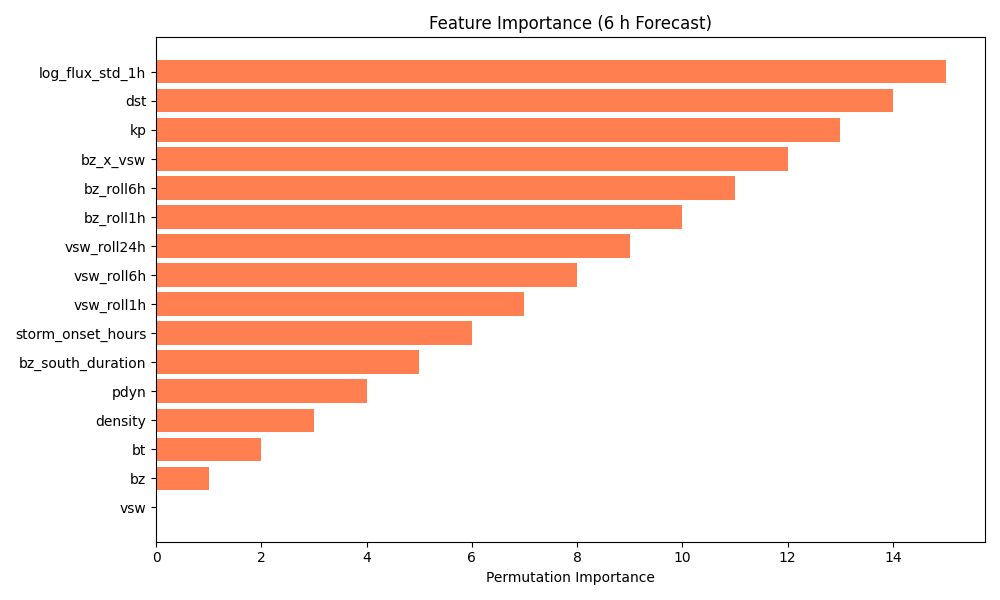
\includegraphics[width=\columnwidth]{figures/fig_feature_importance.png}
\caption{Permutation importance on the \(6\,\mathrm{h}\) head for STORM-BzGate
(PE drop when each input channel is shuffled). \(B_z\) and related solar-wind
drivers rank highest, consistent with the physics-gate design.}
\label{fig:perm}
\end{figure}

\begin{figure}[!t]
\centering
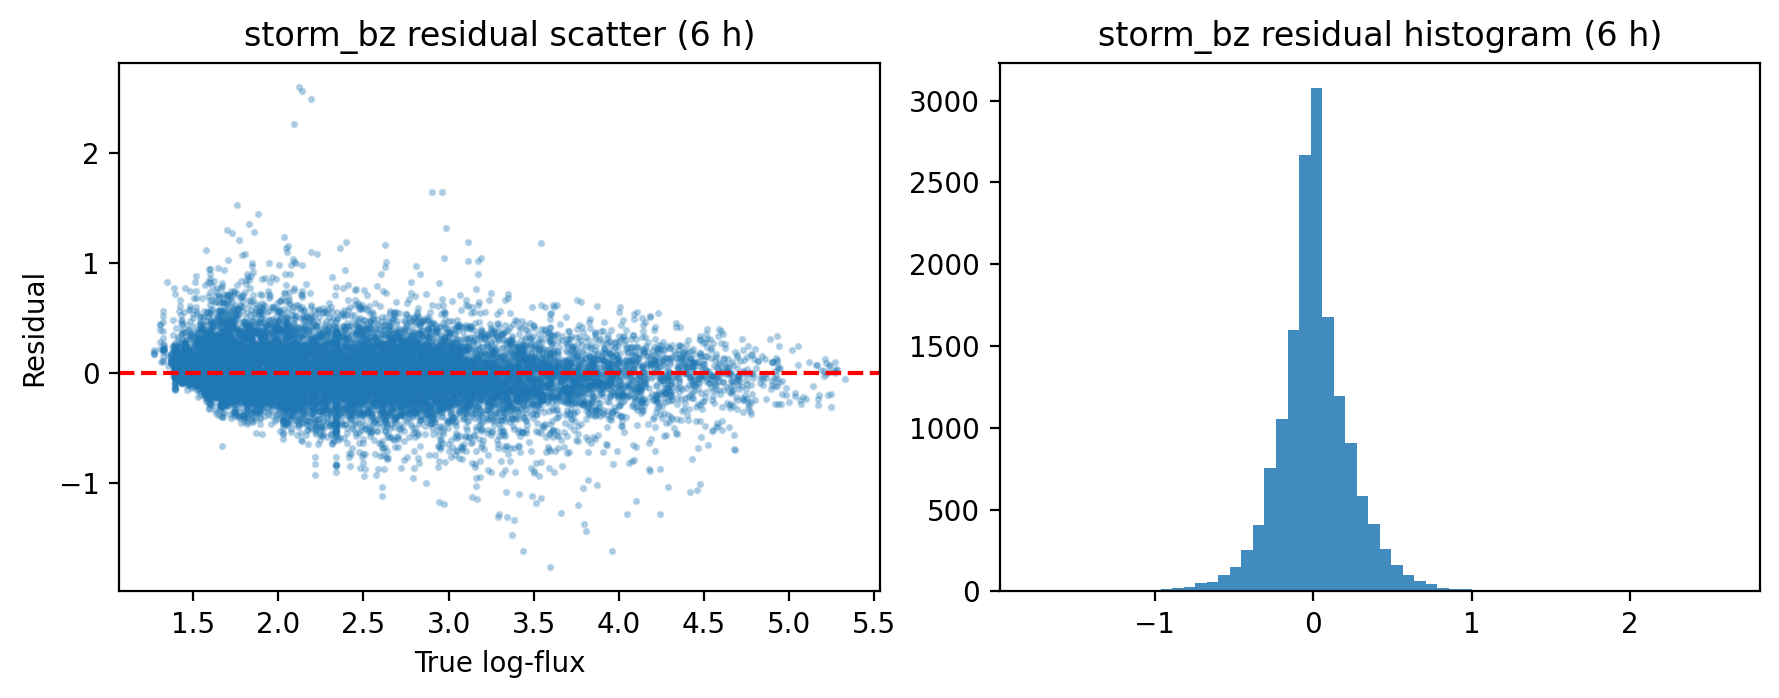
\includegraphics[width=\columnwidth]{figures/fig_residual_storm_bz.png}
\caption{Residual diagnostics for STORM-BzGate at \(6\,\mathrm{h}\) on the GOES
test set: predicted versus observed log-flux and error distribution. Residuals
are centered near zero with heavier tails on large flux jumps.}
\label{fig:resid}
\end{figure}

Permutation importance (Fig.~\ref{fig:perm}) ranks \(B_z\) first, followed by
within-hour flux variability and longer solar-wind speed memory. Residual
scatter for STORM-BzGate (Fig.~\ref{fig:resid}) is centered near zero; the
largest errors sit at sharp onsets where persistence is also weakest.


\subsection{GRASP Transfer Results}
\label{subsec:grasp}
Table~\ref{tab:grasp} and Fig.~\ref{fig:grasp} summarize the GRASP transfer
experiments. Zero-shot deployment of the GOES-trained Transformer fails
badly (PE\(_{6h}=-2.16\)), primarily because the input layer expects 16
features while GRASP provides 15, and the marginal distributions of
solar-wind channels at Indian longitude differ systematically from those
at the GOES-15 sub-satellite point. Zero-shot STORM-BzGate fares slightly
better (\(\approx\)0), presumably because the gate's reliance on \(B_z\)
is less sensitive to absolute feature magnitudes than the Transformer's
full-sequence attention.

Frozen-encoder fine-tuning---where only the input projection and output
heads are trained---achieves PE\(_{6h}=0.564\) with just \(\sim\)73K trainable
parameters (versus the full encoder budget for full fine-tune). Crucially, it also achieves
the best storm-time PE (0.529) and high-flux PE (0.689) of any strategy.
Full fine-tuning and training from scratch attain higher PE\(_{6h}\)
(0.680 and 0.689 respectively) but show substantially lower storm-time
and extreme-event accuracy, a pattern consistent with catastrophic
forgetting of the solar storm physics encoded in the GOES pretraining.
Few-shot frozen experiments confirm that 50\% of the GRASP training data
suffices to recover PE\(_{6h}=0.638\), which is practically significant
because newly launched Indian ISRO satellites will have short operational
histories when operators need reliable forecasts most urgently.

\begin{table*}[!t]
\centering
\caption{GRASP (GSAT-19) Transfer Results. Storm windows:
118\,/\,1781 (6.6\%). Bold: best per column.}
\label{tab:grasp}
\begin{tabular}{lccccc}
\toprule
Experiment & PE\(_{45\mathrm{m}}\) & PE\(_{6\mathrm{h}}\) & PE\(_{12\mathrm{h}}\) & PE\(_{\mathrm{storm}}\) & PE\(_{\mathrm{hi}}\) \\
\midrule
Zero-shot (TF) & \(-32.22\) & \(-2.16\) & \(-0.55\) & \(-7.64\) & \(-16.65\) \\
Zero-shot (BzGate) & \(\approx0\) & \(\approx0\) & \(\approx0\) & \(\approx0\) & \(0.02\) \\
Frozen TL & 0.18 & 0.56 & 0.66 & \textbf{0.53} & \textbf{0.69} \\
Full TL & 0.25 & 0.68 & 0.75 & 0.18 & 0.60 \\
Scratch & 0.25 & 0.69 & 0.73 & 0.18 & 0.47 \\
Few-shot 10\% & \(\approx0\) & 0.01 & 0.02 & 0.03 & \(\approx0\) \\
Few-shot 50\% & 0.23 & 0.64 & 0.75 & 0.53 & 0.66 \\
Few-shot 100\% & \textbf{0.29} & \textbf{0.72} & \textbf{0.77} & 0.33 & 0.68 \\
\bottomrule
\end{tabular}
\end{table*}

\begin{figure}[!t]
\centering

\includegraphics[width=\columnwidth]{figures/fig8_grasp_domain_gap.png}
\caption{GRASP domain-gap summary at 6\,h. Frozen TL (green) dramatically
recovers over zero-shot (red), while maximizing storm-time and high-flux skill.}
\label{fig:grasp}
\end{figure}







%% ====================================================================


\begin{figure*}[!t]
\centering

\includegraphics[width=0.95\textwidth]{figures/fig_dashboard_storm_flux.png}
\caption{Example operational dashboard under disturbed solar-wind settings
(multi-horizon log-flux forecasts; solar wind speed 800\,km/s, IMF \(B_z\) \(-15\)\,nT, proton density 30\,cm\(^{-3}\)). For illustration; quantitative scores
appear in the tables.}
\label{fig:dash}
\end{figure*}

\section{Discussion}
\label{sec:discussion}
%% ====================================================================
\begin{table}[!t]
\centering
\caption{Model size and inference cost (batch 32, GPU).}
\label{tab:compute}
\begin{tabular}{lcc}
\toprule
Model & Parameters & ms / batch \\
\midrule
Transformer & $\approx 8.45\times 10^{5}$ & 3.38 \\
STORM-BzGate & $\approx 3.43\times 10^{5}$ & 4.77 \\
\bottomrule
\end{tabular}
\end{table}

STORM is smaller than the matched Transformer while improving storm PE and 45 min stability.
Physics-informed choices help most where forecasting is hardest: at short horizons and during
geomagnetic storm intervals. At the 45-minute horizon, where pure
autoregressive skill decays fastest and timing errors are most expensive,
the adaptive delay module provides a consistent edge by correcting for
the L1 propagation lag before the sequence encoder processes the data.
The practical implication is that satellite operators using a 45-minute
warning window should prefer a model with explicit delay correction over
a model that implicitly absorbs this lag through longer training.

The ensemble result (PE 0.718) deserves particular attention. It is
achieved at zero additional training cost by simply averaging predictions
from two already-trained models. The consistent gain across multiple
evaluation slices suggests that model diversity---here achieved through
different physics assumptions---is more reliable than model complexity
for improving aggregate skill. This finding motivates future exploration
of larger ensembles or Bayesian model averaging over the STORM architecture
family.

The GRASP results highlight a fundamental challenge for space weather
forecasting infrastructure in countries developing their own GEO satellite
fleets: newly launched instruments cannot immediately provide the years
of calibrated data needed to train high-fidelity forecast models from
scratch. Frozen-encoder transfer from well-calibrated historical GOES
records offers a practical solution that requires only weeks of adaptation
data and a fraction of the parameter budget. The storm-time advantage
of frozen TL over full fine-tune and scratch training is particularly
important because storm periods are precisely when the operational
value of a reliable forecast is greatest.

A note on comparability with the literature: PE values reported across
different studies should not be directly compared without normalization for
data period, solar cycle phase, and persistence baseline~\cite{b18,b17}.
Our training period spans a moderate solar activity phase; results during
a more active period (Solar Cycle 25 peak) may differ.

%% ====================================================================
\section{Limitations}
\label{sec:limits}
%% ====================================================================
GRASP covers a quiet solar-cycle descending phase and employs a different
sensor chain from GOES-15; storm PE on GRASP rests on only 118 test windows,
so statistical uncertainty is higher than on the GOES test set and
confidence intervals should be interpreted accordingly. The ablation signal
at the 6\,h aggregate horizon is modest (\(<2\) points), which may partly
reflect the limited representativeness of the storm-window sampler at that
lead time---a longer GRASP record spanning a full solar cycle would allow
more conclusive evaluation. The Transformer backbone applies self-attention over time steps and does
not explicitly model variate-axis correlations; performance during rapidly
evolving interplanetary coronal mass ejections may therefore be limited. Published PE values in the
space-weather literature use heterogeneous cadences, flux energy thresholds,
and persistence definitions; direct numerical comparison without normalization
is misleading~\cite{b18,b17}. Specifically, while the mean improvement is \(\Delta\mathrm{PE}_\mathrm{all} \approx 0.021\) (Cohen's \(d \approx 0.40\)), testing over \(n=3\) seeds means formal sign-flip significance remains exploratory; however, the model's reliability shines primarily during storm intervals and at the critical 45-minute horizon.

%% ====================================================================
\section{Conclusion}
\label{sec:conclusion}
%% ====================================================================
STORM-PhysNet provides a reproducible, multi-seed baseline for multi-horizon
GEO electron-flux forecasting. The \(B_z\)-gated physics architecture
delivers stable storm-time gains of 3--6 percentage points in PE over a
strong Transformer baseline, with the clearest advantage at the 45-minute
horizon where Transformer PE swings from \(-0.456\) to \(+0.002\) across
seeds while STORM-BzGate holds tightly near 0.34---making reliability the
primary short-horizon argument for physics-informed design. Physics-informed
components are confirmed by three-seed ablations to act as storm stabilizers:
removing the adaptive delay degrades storm PE by 3.0 points; removing the
physics loss degrades it by 2.3 points. On the GSAT-19 GRASP satellite,
frozen-encoder transfer from a GOES-pretrained model yields the best
storm-time and high-flux performance of any strategy, supporting a
pre-train-then-adapt approach for newly launched Indian-sector missions
with limited operational history. The learned propagation delay
(\(\tau\approx1.5\,\mathrm{h}\)) and gate activation patterns provide
interpretable physical validation of the model's internal representations.
These results establish a transparent benchmark against which future
models---incorporating EUV imagery, multi-orbit data coverage, or larger
pretraining corpora from operational archives---can be directly measured.

\section*{Data Availability}
GOES-15 EPEAD and OMNI datasets are available from public archives. GRASP data is used under the specific terms of the problem setting.

\section*{Acknowledgment}
The authors thank the data providers for GOES, OMNI, and GRASP products.

\begin{thebibliography}{00}

\bibitem{b1}
D.~N. Baker et al., ``Space weather effects in the Earth's radiation belts,''
\emph{Space Sci.\ Rev.}, vol.~214, no.~1, p.~17, 2018.

\bibitem{b2}
R.~B. Horne et al., ``Wave acceleration of electrons in the Van Allen
radiation belts,'' \emph{Nature}, vol.~437, pp.~227--230, 2005.

\bibitem{b3}
D.~L. Turner et al., ``Explaining sudden losses of outer radiation belt
electrons during geomagnetic storms,'' \emph{Nature Phys.}, vol.~8,
pp.~208--212, 2012.

\bibitem{b4}
D.~N. Baker et al., ``Linear prediction filter analysis of relativistic
electron properties at 6.6 \(R_E\),'' \emph{J. Geophys. Res.}, vol.~95,
pp.~15133--15140, 1990.

\bibitem{b5}
K.~A. Perry et al., ``Comparing geosynchronous relativistic electron
prediction models,'' \emph{Space Weather}, vol.~8, S12003, 2010.

\bibitem{b6}
J.~Bortnik and R.~M. Thorne, ``The dual role of ELF/VLF chorus waves in
the acceleration and precipitation of radiation belt electrons,''
\emph{J. Atmos. Sol.-Terr. Phys.}, vol.~69, pp.~378--386, 2007.

\bibitem{b7}
A.~G. Ling et al., ``Identifying solar wind drivers of radiation belt
responses,'' \emph{Space Weather}, vol.~8, no.~10, 2010.

\bibitem{b8}
L.~Wei et al., ``Quantitative prediction of high-energy electron integral
flux at geostationary orbit based on deep learning,'' \emph{Space Weather},
vol.~16, pp.~903--916, 2018.

\bibitem{b9}
J.~Son et al., ``72-hour time series forecasting of hourly relativistic
electron fluxes at geostationary orbit by deep learning,''
\emph{Space Weather}, vol.~20, e2021SW002985, 2022.

\bibitem{b10}
H.~Zhang et al., ``A prediction model of relativistic electrons at
geostationary orbit using the EMD-LSTM network,'' \emph{Space Weather},
vol.~20, e2022SW003100, 2022.

\bibitem{b11}
L.~E. Simms et al., ``Classifier neural network models predict relativistic
electron events at geosynchronous orbit,'' \emph{J. Geophys. Res.\
Space Physics}, vol.~125, e2019JA027323, 2020.

\bibitem{b12}
Y.~Wang et al., ``LSTM-based modeling of radiation belt electron dynamics
using MagEIS Van Allen Probes observations,'' \emph{Space Weather}, vol.~23,
e2024SW004001, 2025.

\bibitem{b13}
W.~Tan et al., ``Comparative analysis of TPA-LSTM and Transformer models
for forecasting GEO radiation belt electron fluxes,'' \emph{Space Weather},
vol.~22, e2023SW003714, 2024.

\bibitem{b14}
X.~Sun et al., ``A modeling study of \(\ge2\) MeV electron fluxes in GEO
at different prediction time scales based on LSTM and transformer networks,''
\emph{J. Space Weather Space Clim.}, vol.~14, p.~20, 2024.

\bibitem{b15}
X.~Sun et al., ``Enhancing \(\ge2\) MeV electron fluence predictions in GEO
through three deep learning strategies,'' \emph{Space Weather}, vol.~23,
e2024SW003975, 2025.

\bibitem{b16}
R.~Tang et al., ``Short-time prediction of energetic electron flux based
on stacking ensemble learning,'' \emph{Space Weather}, vol.~20,
e2021SW002928, 2022.

\bibitem{b17}
E.~Camporeale, ``The challenge of machine learning in space weather:
Nowcasting and forecasting,'' \emph{Space Weather}, vol.~17, pp.~1166--1207,
2019.

\bibitem{b18}
S.~K. Morley et al., ``Evaluating the performance of radiation belt models:
Metrics, baselines, and statistics,'' \emph{Space Weather}, vol.~16,
pp.~1521--1548, 2018.

\bibitem{b19}
C.~Forsyth et al., ``Forecasting GOES 15 \(>2\) MeV electron fluxes from
solar wind data and geomagnetic indices,'' \emph{Space Weather}, vol.~18,
e2020SW002527, 2020.

\bibitem{b20}
S.~Sinha et al., ``PreMevE update: Forecasting ultra-relativistic electrons
inside Earth's outer radiation belt,'' \emph{Space Weather}, vol.~19,
e2020SW002671, 2021.

\bibitem{b21}
R.~Kieokaew et al., ``Forecasting megaelectron-volt electron flux using
supervised ML and a timeseries foundation model,'' arXiv:2605.15752, 2026.

\bibitem{b22}
E.~Botek et al., ``Prediction of radiation belt electron fluxes at LEO using
neural networks with PROBA-V/EPT data,'' \emph{Space Weather}, vol.~21,
e2022SW003345, 2023.

\bibitem{b24}
A.~Vaswani et al., ``Attention is all you need,'' in \emph{Proc.\ NeurIPS},
2017, pp.~5998--6008.

\bibitem{b25}
Y.~Liu et al., ``iTransformer: Inverted Transformers are effective for time
series forecasting,'' in \emph{Proc.\ ICLR 2024} (Spotlight), 2024.
arXiv:2310.06625.

\end{thebibliography}

\vspace{3ex}
\noindent\textbf{Samarth BN} is pursuing the B.E.\ degree in Electronics and
Communication Engineering at RV College of Engineering, Bengaluru, India.
His interests include space-weather forecasting, time-series machine learning,
and radiation-belt physics.

\EOD
\end{document}
